%++++++++++++++++++++++++++++++++++++++++
% Don't modify this section unless you know what you're doing!
\documentclass[letterpaper,12pt]{article}
\usepackage{tabularx} % extra features for tabular environment
\usepackage{amsmath}  % improve math presentation
\usepackage{mathabx}
\usepackage{braket}
\usepackage{siunitx}
\usepackage{graphicx} % takes care of graphic including machinery
\usepackage[margin=1in,letterpaper]{geometry} % decreases margins
\usepackage{cite} % takes care of citations
\usepackage[final]{hyperref} % adds hyper links inside the generated pdf file
\usepackage{blkarray}
\usepackage{multirow}
\usepackage{tikz}
\usetikzlibrary{calc}
\hypersetup{
	colorlinks=true,       % false: boxed links; true: colored links
	linkcolor=blue,        % color of internal links
	citecolor=blue,        % color of links to bibliography
	filecolor=magenta,     % color of file links
	urlcolor=blue         
}
%++++++++++++++++++++++++++++++++++++++++


\begin{document}

\title{Report IV}
\author{Cristina Mier Gonz\'alez}
\date{\today}
\maketitle

\begin{abstract}
Explain Rashba Hamiltonian, write explicit matrix. Some results in dimer and atomic chain.
\end{abstract}

\section{Spin-orbit coupling: Rashba Hamiltonian}
For a flat surface, with an electric field perpendicular to the $xy$ plane, the Rashba Hamiltonian is written \cite{Manchon2015}:
\begin{equation}
    \hat{H}_{Rashba} = \frac{\alpha_R}{\hbar}(\Vec{\sigma}\times\Vec{p})_z
\end{equation}
Where $\alpha_R$ is the spin-orbit coupling strength and $\Vec{\sigma} = (\sigma_x, \sigma_y, \sigma_z)$ are the spin Pauli matrices. In a 2D system, where electrons are confined in the $xy$ plane, the Rashba Hamiltomian becomes:
\begin{equation}
    \hat{H}_{Rashba} = \frac{\alpha_R}{\hbar}(p_y\sigma_x - p_x\sigma_y)
    \label{2D}
\end{equation}
The momentum operator is related to the differential operator:
\begin{equation}
    \hat{p}_x = -i\hbar\frac{\partial}{\partial x} \qquad \hat{p}_y = -i\hbar\frac{\partial}{\partial y}
\end{equation}
Using finite differences and the following discretization of the 2D space in $\ket{n, m} = \ket{x = na, y = ma}$ where $a$ is the lattice parameter, the momentum operators become,\cite{thesis}:
\begin{equation}
    \hat{p}_x = -i\hbar \frac{\ket{n+1, m}\bra{n, m}}{2a} \qquad  \hat{p}_y = -i\hbar \frac{\ket{n, m+1}\bra{n, m}}{2a}
\end{equation}
The Rashba Hamiltonian is now given:
\begin{equation}
    \hat{H}_{Rashba} = \frac{\alpha_R}{2a}\sum_{n, m, \sigma}\Bigg[ \big(\ket{n+1, m}_\sigma\bra{n, m}_{\sigma'}\times i\sigma_y\big) - \big(\ket{n, m+1}_{\sigma}\bra{n, m}_{\sigma'}\times i\sigma_x \big)\Bigg] + h.c.
     \label{tight}
\end{equation}
The subindex $\sigma$ indicates the spin of each state. The Hamiltonian couples states at nearest neighbours sites and with different spin state. \\ \\
%We want to write Equation \ref{tight} in matrix form using the Nambu basis $\Psi = [\psi_\uparrow \psi_\downarrow \psi_\uparrow^\dagger \psi_\downarrow^\dagger]^T$. For the coupling along the $x$ direction we have:
$\sigma_x$ and $\sigma_y$ are two-dimension matrices covering the two spin states $\uparrow$ and $\downarrow$. 
However, we want to write equation \ref{tight} using the four-component Nambu basis: $\Psi = [\psi_\uparrow \psi_\downarrow \psi_\uparrow^\dagger \psi_\downarrow^\dagger]^T$, where the two last terms correspond to the time-reversed components. 
\begin{equation}
\footnotesize
\hat{H}_{Rashba} = \frac{\alpha_R}{2a}
    \begin{pmatrix}
    0 & \hat{p}_x - i\hat{p}_y\quad\hat{p}_x^\dagger + i\hat{p}_y^\dagger & 0 & 0\\
    -\hat{p}_x + i\hat{p}_y\quad-\hat{p}_x^\dagger - i\hat{p}_y^\dagger & 0 & 0 & 0\\
    0 & 0 & 0 & -\hat{p}_x + i\hat{p}_y\quad-\hat{p}_x^\dagger - i\hat{p}_y^\dagger\\
    0 & 0 & \hat{p}_x - i\hat{p}_y\quad\hat{p}_x^\dagger + i\hat{p}_y^\dagger & 0
    \end{pmatrix}
\end{equation}

Where the upper block correspond to the electron space and the lower block is the time-reversed or hole space. The timer reversed Hamiltonian is defined as minus the complex conjugate, this is, $ - \hat{H}^\dagger$. Nevertheless, when writing this matrix for the superconducting array of dimension $N_x \times N_y$, I need to differentiate between the Rashba coupling in the $x$ and $y$ direction.\\ \\
To understand this issue, I will explicitly write the matrix of the Rashba interaction, for the case where $N_x = 2$ and $N_y = 3$.\\ \\
\begin{figure}[h!]
\centering
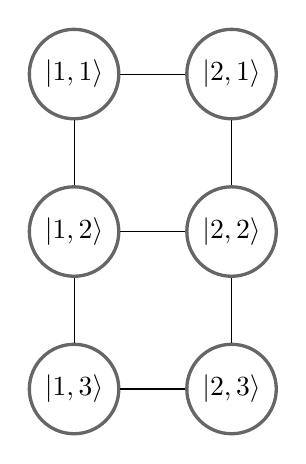
\begin{tikzpicture}[node distance=2cm, roundnode/.style={circle, draw=black!60, very thick, minimum size=7mm},]  
\node[roundnode](1)                      {$\ket{1,1}$};
\node[roundnode](2)         [right of=1]{$\ket{2,1}$};
\node[roundnode](3)         [below of=1]{$\ket{1,2}$};
\node[roundnode](4)                      [below of=2]{$\ket{2,2}$};
\node[roundnode](5)                      [below of=3]{$\ket{1,3}$};
\node[roundnode](6)                      [below of=4]{$\ket{2,3}$};

\draw(1) -- (2);
\draw(1) -- (3);
\draw(2) -- (4);
\draw(3) -- (4);
\draw(1) -- (3);
\draw(3) -- (5);
\draw(4) -- (6);
\draw(5) -- (6);

\end{tikzpicture} 
\label{diagram}
\caption{\footnotesize Lattice with $N_x = 2$ and $N_y = 3$ resulting in 6 sites lattice, labelled using the notation $\ket{n, m}$.}
\end{figure}

The resulting matrix will have total size $24 \times 24$, because the lattice has 6 sites times the 4 Nambu components.
\[
\renewcommand\arraystretch{1.75}
\footnotesize
\begin{blockarray}{rccccccccc}
&&& \ket{1, 1} & \ket{2, 1} & \ket{1, 2} & \ket{2, 2} & \ket{1, 3} & \ket{2, 3} &\\
\begin{block}{rc[c@{}c|c|c|c|c|c@{}c]}
  & \bra{1, 1} &&  & \hat{H}_x & \hat{H}_y &  &  & &\vphantom{\smash[b]{\bigg|}} \\
\BAhhline{~~~------~}
  & \bra{2,1} && \hat{H}_x^\dagger &  & & \hat{H}_y  &  & &\\
\BAhhline{~~~------~}
\hat{H}_{Rashba}=\quad
 & \bra{1,2} &&  \hat{H}_y^\dagger  &  &  &  \hat{H}_x &  \hat{H}_y  & &\\
\BAhhline{~~~------~}
  & \bra{2,2} &&  &  \hat{H}_y^\dagger  &  \hat{H}_x^\dagger  &  &   & \hat{H}_y \\
\BAhhline{~~~------~}
 & \bra{1,3} &&  &  &  \hat{H}_y^\dagger &  &  &  \hat{H}_x &\\
 \BAhhline{~~~------~}
  & \bra{2,3} &&  &  &  & \hat{H}_y^\dagger & \hat{H}_x^\dagger  & \vphantom{\smash[t]{\bigg|}} &\\
\end{block}
\end{blockarray}
\]
Each of the sites of the previous matrix has actually size $4\times 4$. As we can see, the Rashba Hamiltonian has been divided between $x$ and $y$ coupling. The $\hat{H}_x$ and $\hat{H}_y$ are given:


\begin{equation}
\hat{H}_x = 
    \frac{\alpha_R}{2a}\begin{pmatrix}
    0 & 1 & 0 & 0 \\
    -1 & 0 & 0 & 0 \\
    0 & 0 & 0 & -1 \\
    0 & 0 & 1 & 0
  \end{pmatrix}
\end{equation}
\vspace{0.5cm}
\begin{equation}
\hat{H}_y = 
    \frac{\alpha_R}{2a}\begin{pmatrix}
    0 & -i & 0 & 0 \\
    -i & 0 & 0 & 0 \\
    0 & 0 & 0 & -i \\
    0 & 0 & -i & 0
  \end{pmatrix}
\end{equation}
The Rashba Hamiltonian is added to the Self energy matrix, $\Sigma$ ,as a perturbation to the BCS Hamiltonian. The Green's function of the total system which allows us to obtain the spectrum is obtained by solving Dyson's equation:
\begin{equation}
    G = [1 - G_o\Sigma]^{-1}G_o
\end{equation}

\section{Results}
Using the program introduced in previous reports, the chain of adatoms on the supercondcuting matrix, I performed several simulations for different chain lengths. Here I summarize the most interesting results for the dimer and the long atomic chain.

\subsection{Dimer}
The dimer results were already summarize in Report I. However, improvements in the representation allows for a better visualization of the effect of the potential scattering as well as the effect of the SOC.\\ \\
In the case of a dimer, the size of the superconductor underneath the magnetic atoms, has not a big effect on the resulting spectrum. Like this, the simulations are performed taking a lattice of size $N_x = 4$ amd $N_y$ 



   
 

\bibliography{name.bib}{}
\bibliographystyle{abbrv}


\end{document}
